\chapter{System Architecture}

This paper proposes a high-performance data center system architecture based on programmable network cards. As shown in Figure \ref{arch:fig:virt-architecture}, this paper upgrades ordinary network cards to programmable network cards, offloads the high-performance data plane required by virtualization, network and storage functions, and the operating system to the programmable network card, in order to reduce the "data center tax" and allow the CPU to focus on the client's applications.

\begin{figure}[htbp]
	\centering
	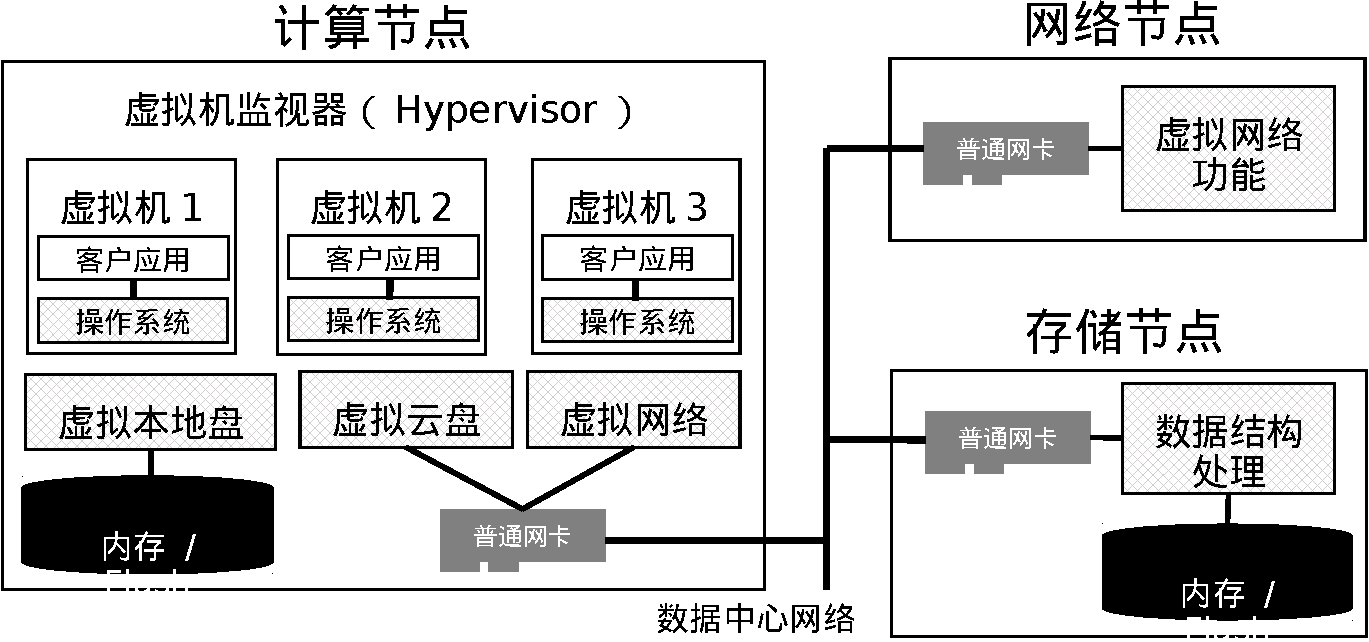
\includegraphics[width=0.8\textwidth]{figures/virt_arch.pdf}
	\caption{Review: Data center architecture with virtualization.}
	\label{arch:fig:virt-architecture}
\end{figure}

As discussed in Chapter \ref{chapter:intro}, a virtualized data center can mainly be divided into computing, network, and storage nodes. In network and storage nodes, a design concept of separating the control plane from the data plane is adopted. The data plane handles relatively frequent and simple operations, while the control plane handles relatively infrequent and complex operations. The data plane is implemented in the programmable network card, and the control plane is implemented on the host CPU, achieving a data plane that does not pass through the host CPU at all. This includes the virtual network functions in Chapter \ref{chapter:clicknp} and the data structure processing in Chapter \ref{chapter:kvdirect}. Accelerating virtual network functions and remote data structure access are also the most important innovations of this paper.

In the computing node, that is, the server host where the client virtual machine is located, the programmable network card implements the virtualization functions of the virtual machine monitor (hypervisor) and the operating system primitives. Virtualization is divided into "one-to-many" and "many-to-one" aspects. "One-to-many" means that the programmable network card virtualizes the hardware resources within the computing node into multiple logical resources, achieving multiplexing of other computing nodes and multiple local virtual machines. For example, ClickNP in Chapter \ref{chapter:clicknp} virtualizes the hardware network card and network link into a virtual network card for each virtual machine; KV-Direct in Chapter \ref{chapter:kvdirect} allows multiple clients to concurrently access shared key-value storage while ensuring consistency. "Many-to-one" means that the programmable network card virtualizes physically dispersed resources within the data center into a logical resource, achieving mapping and routing from logical resources to physical resources. For example, ClickNP in Chapter \ref{chapter:clicknp} virtualizes network functions within the data center into logically unified network functions; the KV-Direct client in Chapter \ref{chapter:kvdirect} virtualizes distributed key-value storage into logically unified key-value mapping; it can also achieve disaggregation of storage and memory. In order to accelerate operating system primitives and control hardware complexity, operating system primitives are divided into reliable communication protocols on the programmable network card and user-space libraries and user-space management programs running on the host CPU, such as the socket communication primitives implemented by SocksDirect in Chapter \ref{chapter:socksdirect}.

Figure \ref{arch:fig:accel-arch} shows the overall architecture of the system based on the programmable network card. The overall design of the subsequent chapters of this paper will be briefly introduced in the order of network, storage, and high-level abstraction.

\begin{figure}[htbp]
	\centering
	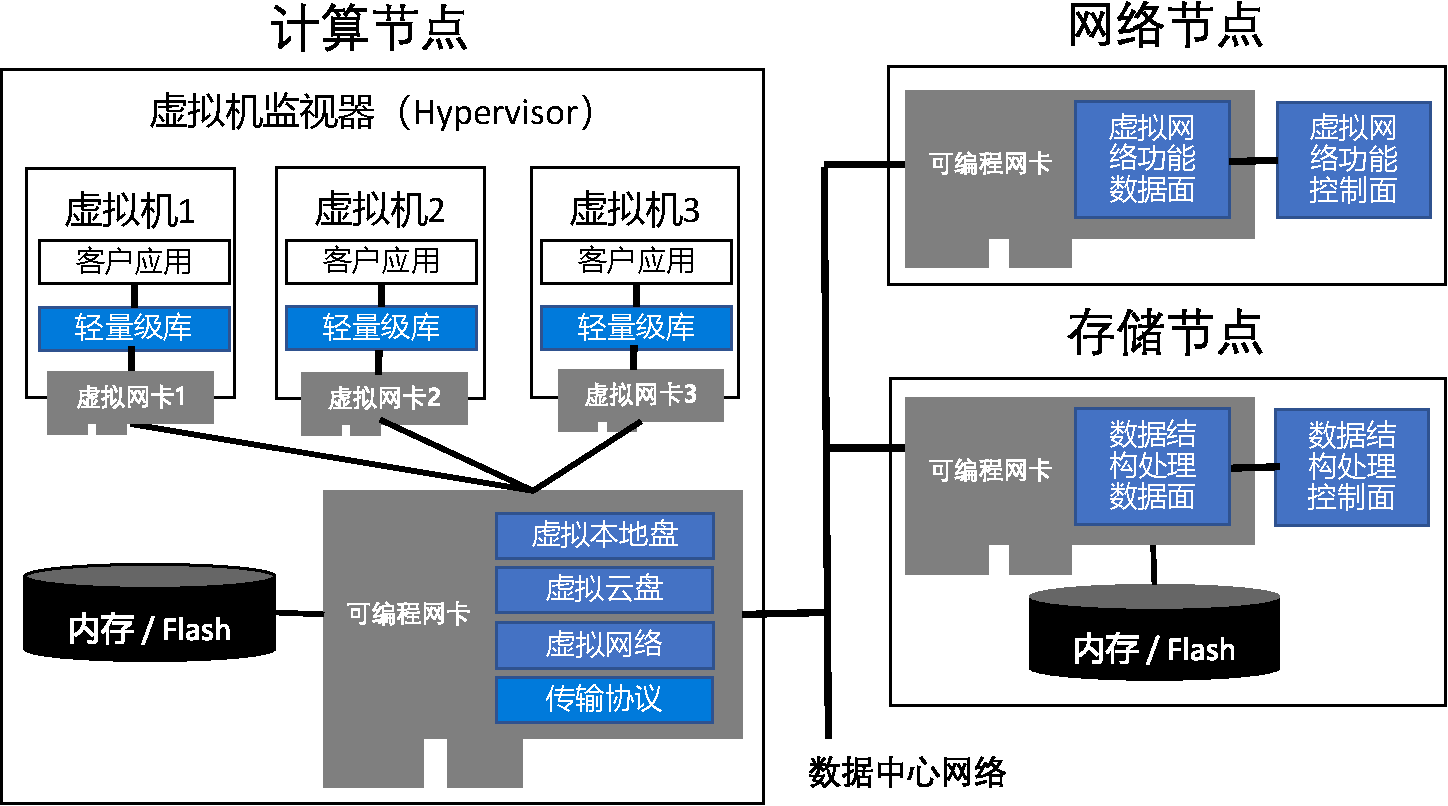
\includegraphics[width=0.8\textwidth]{figures/accel_arch.pdf}
	\caption{Overall architecture of the data center system based on the programmable network card.}
	\label{arch:fig:accel-arch}
\end{figure}

\section{Network Acceleration}

\subsection{Network Virtualization Acceleration}

Starting from the traditional data center architecture in Chapter \ref{chapter:intro} (Figure \ref{intro:fig:virt-architecture}), this paper gradually eliminates or offloads the "data center tax" to the programmable network card. As shown in Figure \ref{arch:fig:virtual-network}, the first step is to replace the original ordinary network card with a programmable network card and offload the software-implemented virtual network to the programmable network card.

\begin{figure}[htbp]
	\centering
	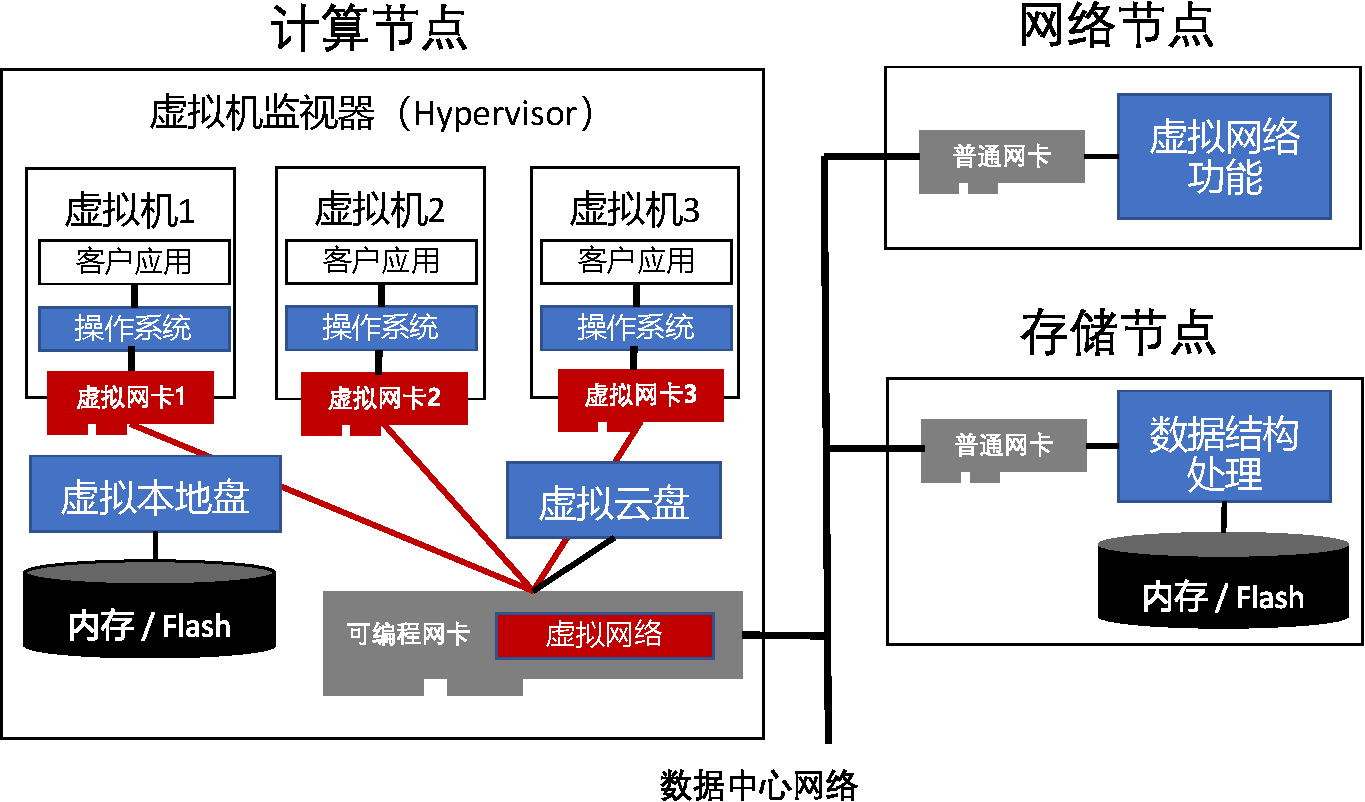
\includegraphics[width=0.8\textwidth]{figures/virtual_network.pdf}
	\caption{Architecture after accelerating the virtual network with a programmable network card.}
	\label{arch:fig:virtual-network}
\end{figure}

In order for the operating system network protocol stack on the virtual machine to use the virtual network to send and receive data packets, the programmable network card uses SR-IOV (Single Root I/O Virtualization) technology \cite{dong2012high} to virtualize into multiple PCIe virtual devices (VF, Virtual Function), and assigns a PCIe virtual device to each virtual machine. The original virtual network card driver in the virtual machine (such as those based on virtio technology \cite{russell2008virtio}) needs to be replaced with the FPGA driver and FPGA-based virtual network card driver implemented in this paper. ClickNP in Chapter \ref{chapter:clicknp} virtualizes the hardware network card and network link into the virtual network of multiple tenants.

If we can bypass the network protocol stack of the virtual machine operating system and directly replace the standard library (i.e., system call interface libc) used by the application program on the virtual machine, there is no need to implement SR-IOV hardware virtualization.
Chapter \ref{chapter:socksdirect} of SocksDirect intercepts the standard library calls about network sockets of the application program and implements the container overlay network (suitable for container virtual network) in user mode.
For efficient communication between the user mode runtime library and the programmable network card, the FPGA driver is installed in the virtual machine, and a part of the PCIe address space of the programmable network card is mapped to the user mode, thereby bypassing the virtual machine kernel and the Virtual Machine Monitor or Hypervisor.

\subsection{Network Function Acceleration}

As shown in Figure \ref{arch:fig:network-function}, the second step is to divide the software-implemented virtual network function into a data plane and a user plane on the network node, and unload the data plane into the programmable network card.
It should be noted that the division of network nodes and computing nodes is logical. It is possible that the virtual network function is orchestrated to the same server host as the virtual machine, at which time the functions of the network node and the computing node are combined into one, and the connection between the virtual network and the virtual network function is simplified from the data center network to the connection between modules in the programmable network card.

After the data packet from the source computing node (or the previous network node) is received by the programmable network card of the network node, it is processed in the data plane of the network card. In most cases, the control plane on the CPU does not need to be involved, and the processed data packet can be sent back to the data center network, reaching the destination computing node (or the next network node).
Chapter \ref{chapter:clicknp} will introduce how to use high-level language modular programming to implement network functions, and implement the collaborative processing of the FPGA data plane and the CPU control plane.

\begin{figure}[htbp]
	\centering
	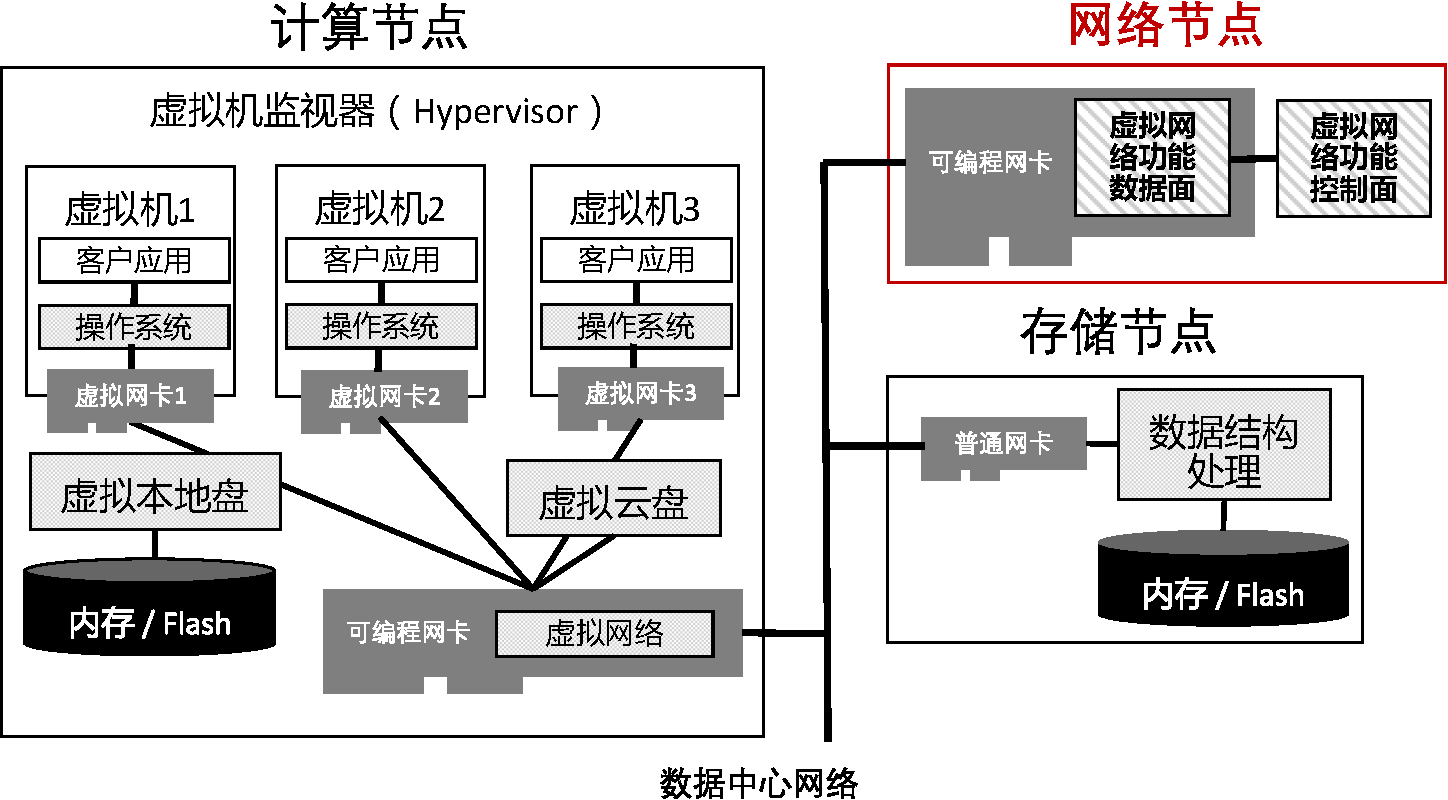
\includegraphics[width=0.8\textwidth]{figures/NFV_accel.pdf}
	\caption{Architecture after accelerating network functions with a programmable network card.}
	\label{arch:fig:network-function}
\end{figure}

\section{Storage Acceleration}

\subsection{Storage Virtualization Acceleration}

After network acceleration, the third and fourth steps are storage acceleration. As the third step, the storage virtualization function of the computing node is first offloaded to the programmable network card, as shown in Figure \ref{arch:fig:virt-storage} \footnote{This paper does not make contributions in the area of storage virtualization, it is included in the system architecture for completeness.}.

To support distributed storage composed of multiple storage nodes, the virtual cloud storage service needs to map logical addresses to storage node addresses. For example, in the distributed key-value storage in Chapter \ref{chapter:clicknp}, the client needs to map the key to the storage node according to consistent hashing \cite{nishtala2013scaling}, and then route the request to that node.

\begin{figure}[htbp]
	\centering
	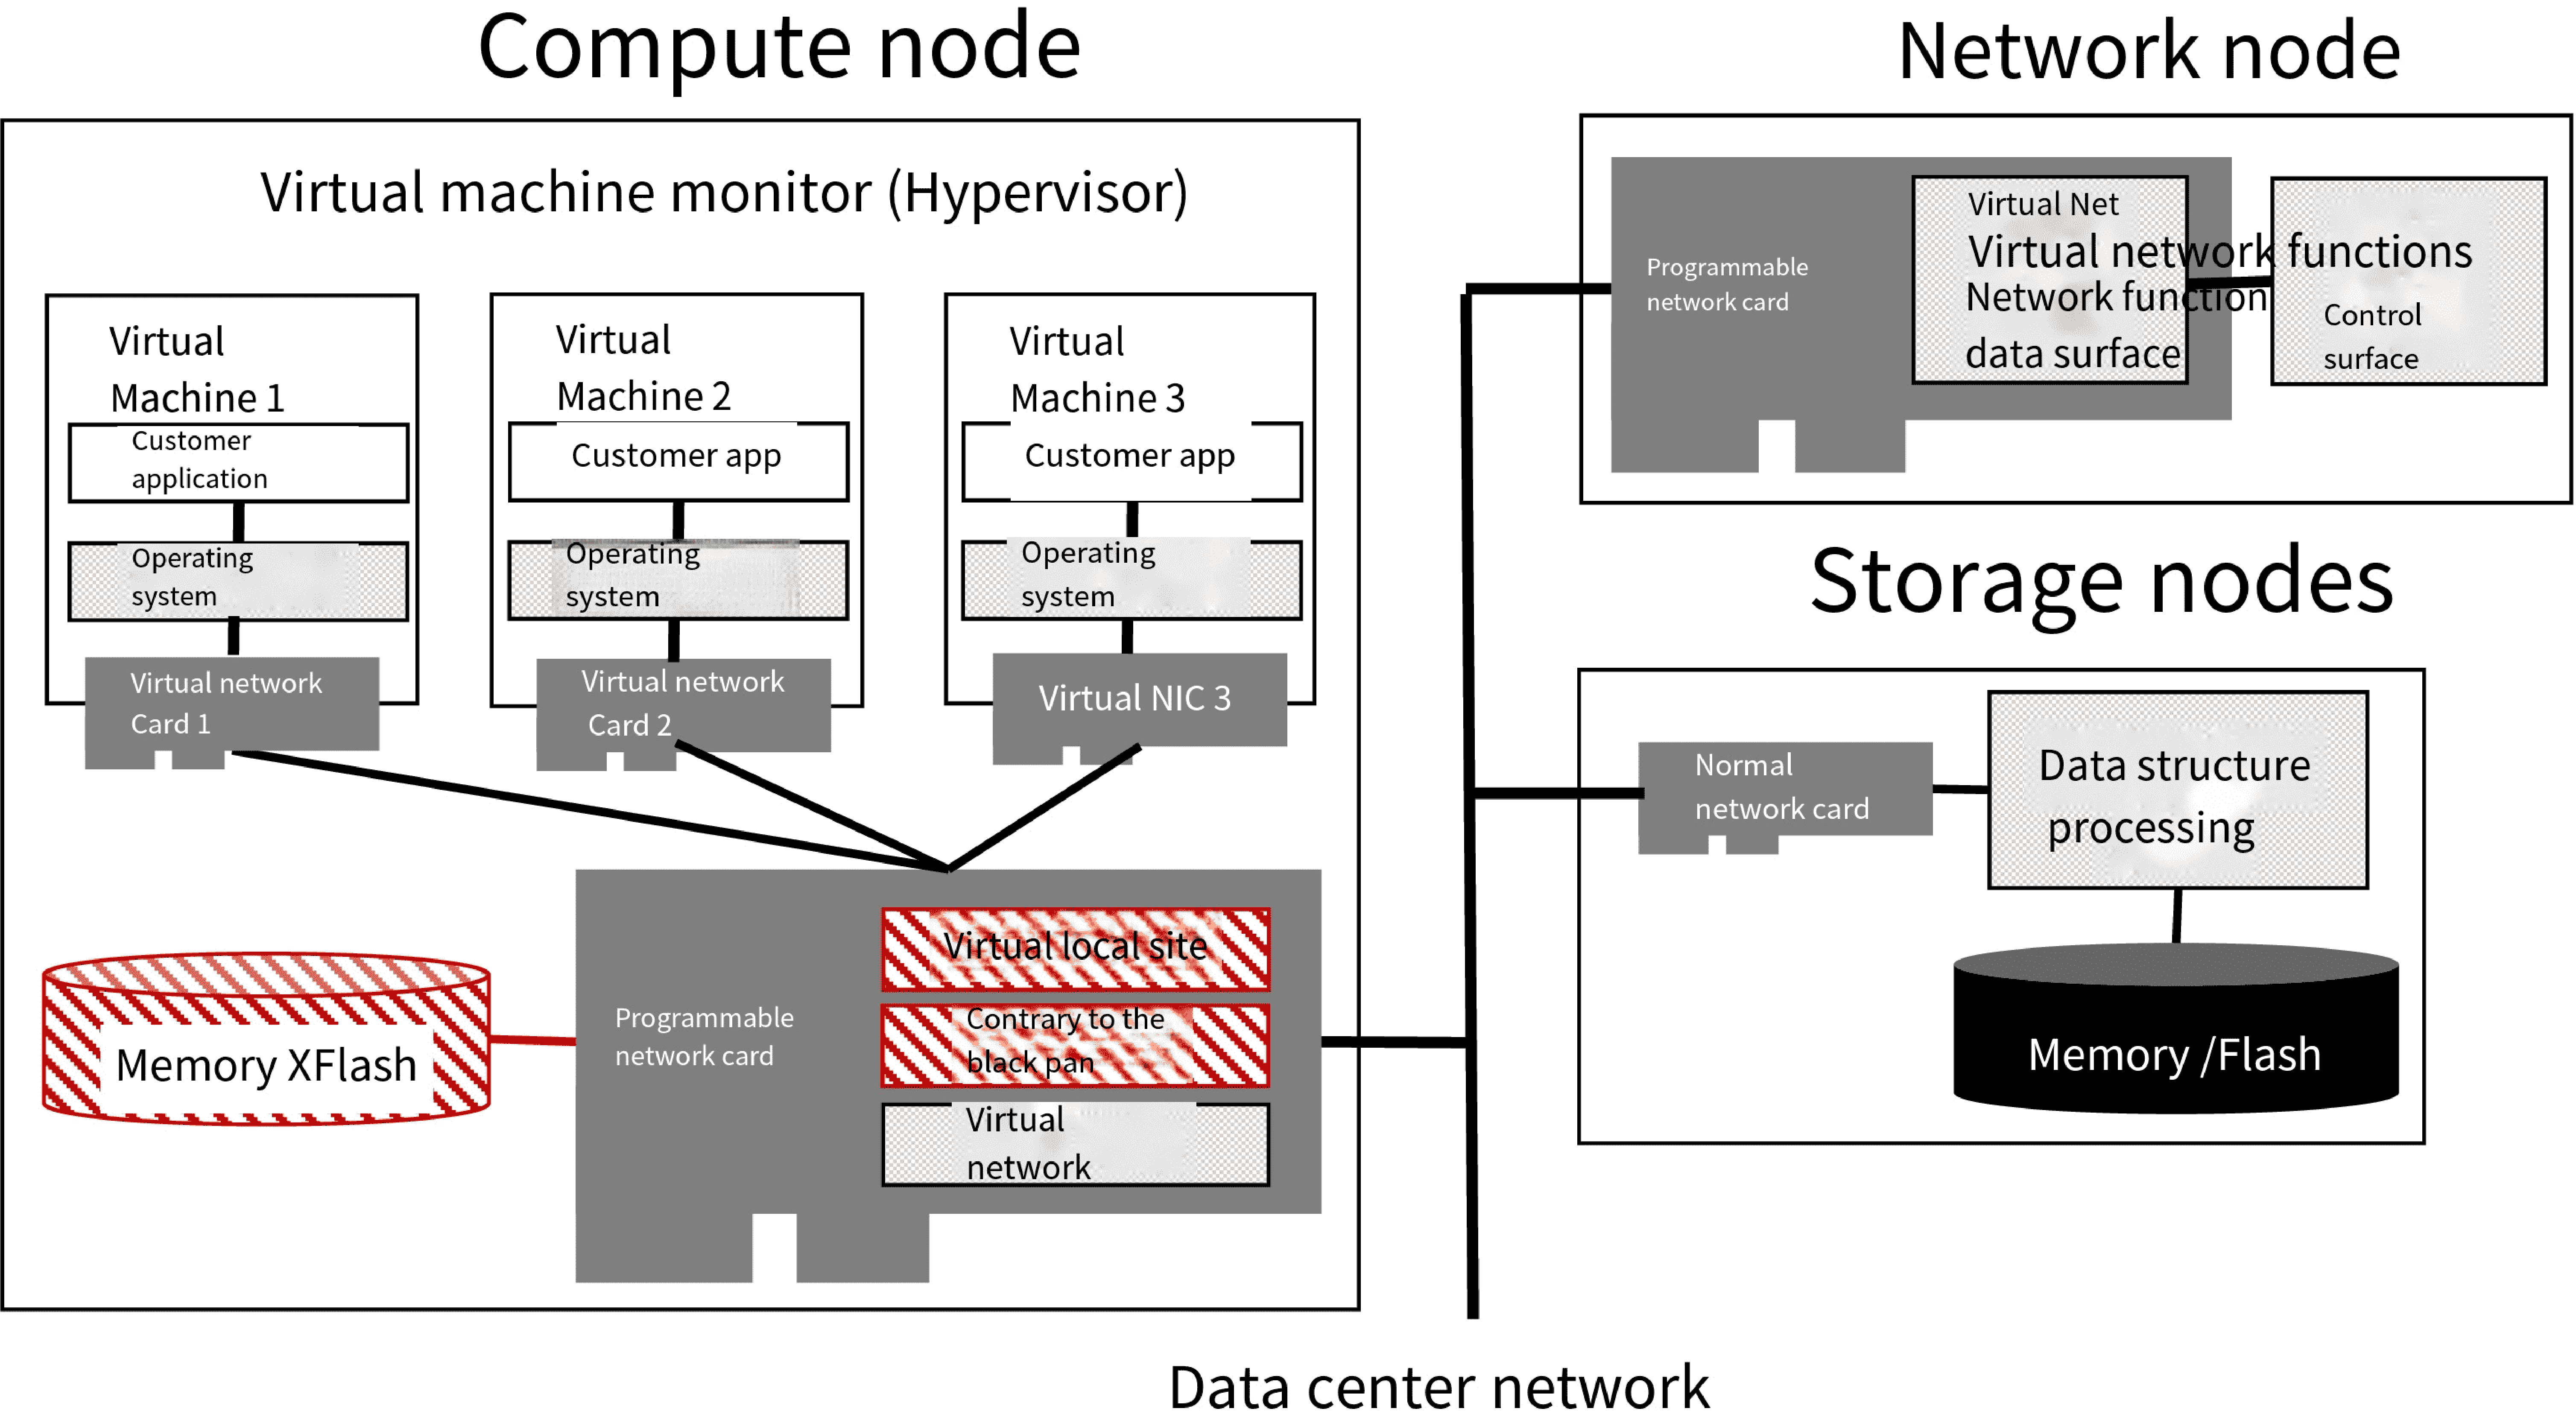
\includegraphics[width=0.8\textwidth]{figures/virt_storage.pdf}
	\caption{Architecture after accelerating local storage and cloud storage with a programmable network card.}
	\label{arch:fig:virt-storage}
\end{figure}

\subsection{Data Structure Processing Acceleration}

The fourth step is to offload the data structure processing on the storage node to the programmable network card.
Take the key-value storage detailed in Chapter \ref{chapter:kvdirect} as an example.
After the programmable network card on the storage node receives a request to query (GET) or write (PUT) a certain key from the network, it needs to query the corresponding key-value pair from the local memory or flash memory, process the request, and then send the result to the requester on the network.
As shown in Figure \ref{arch:fig:data-structure-accel}, this process is called the data plane of data structure processing, and usually does not require the intervention of the control plane.
However, since complex logic is not suitable for running on the programmable network card, the memory allocator is divided into two parts: the network card and the host CPU. The network card caches several fixed-size free memory blocks. When the free memory blocks are insufficient, the control plane on the host CPU needs to supplement the free memory blocks by splitting larger memory blocks; when there are too many free memory blocks, the host CPU needs to perform garbage collection and merge into larger memory blocks.
Another challenge of directly accessing memory data structures through the network card is the lower PCIe bandwidth and higher latency between the network card and memory. For this, Chapter \ref{chapter:kvdirect} designed a series of optimization methods to save bandwidth and hide latency through concurrent processing.
Despite the concurrent processing of requests, the design of Chapter \ref{chapter:kvdirect} can still ensure the strong consistency of concurrent access by multiple clients, that is, the requests are logically processed in the order they are received by the network.
If the storage node also runs a virtual machine as a computing node, in order to solve the consistency problem when accessing the same storage area locally and remotely, whether it is local or remote access, it is processed through the programmable network card.

\begin{figure}[htbp]
	\centering
	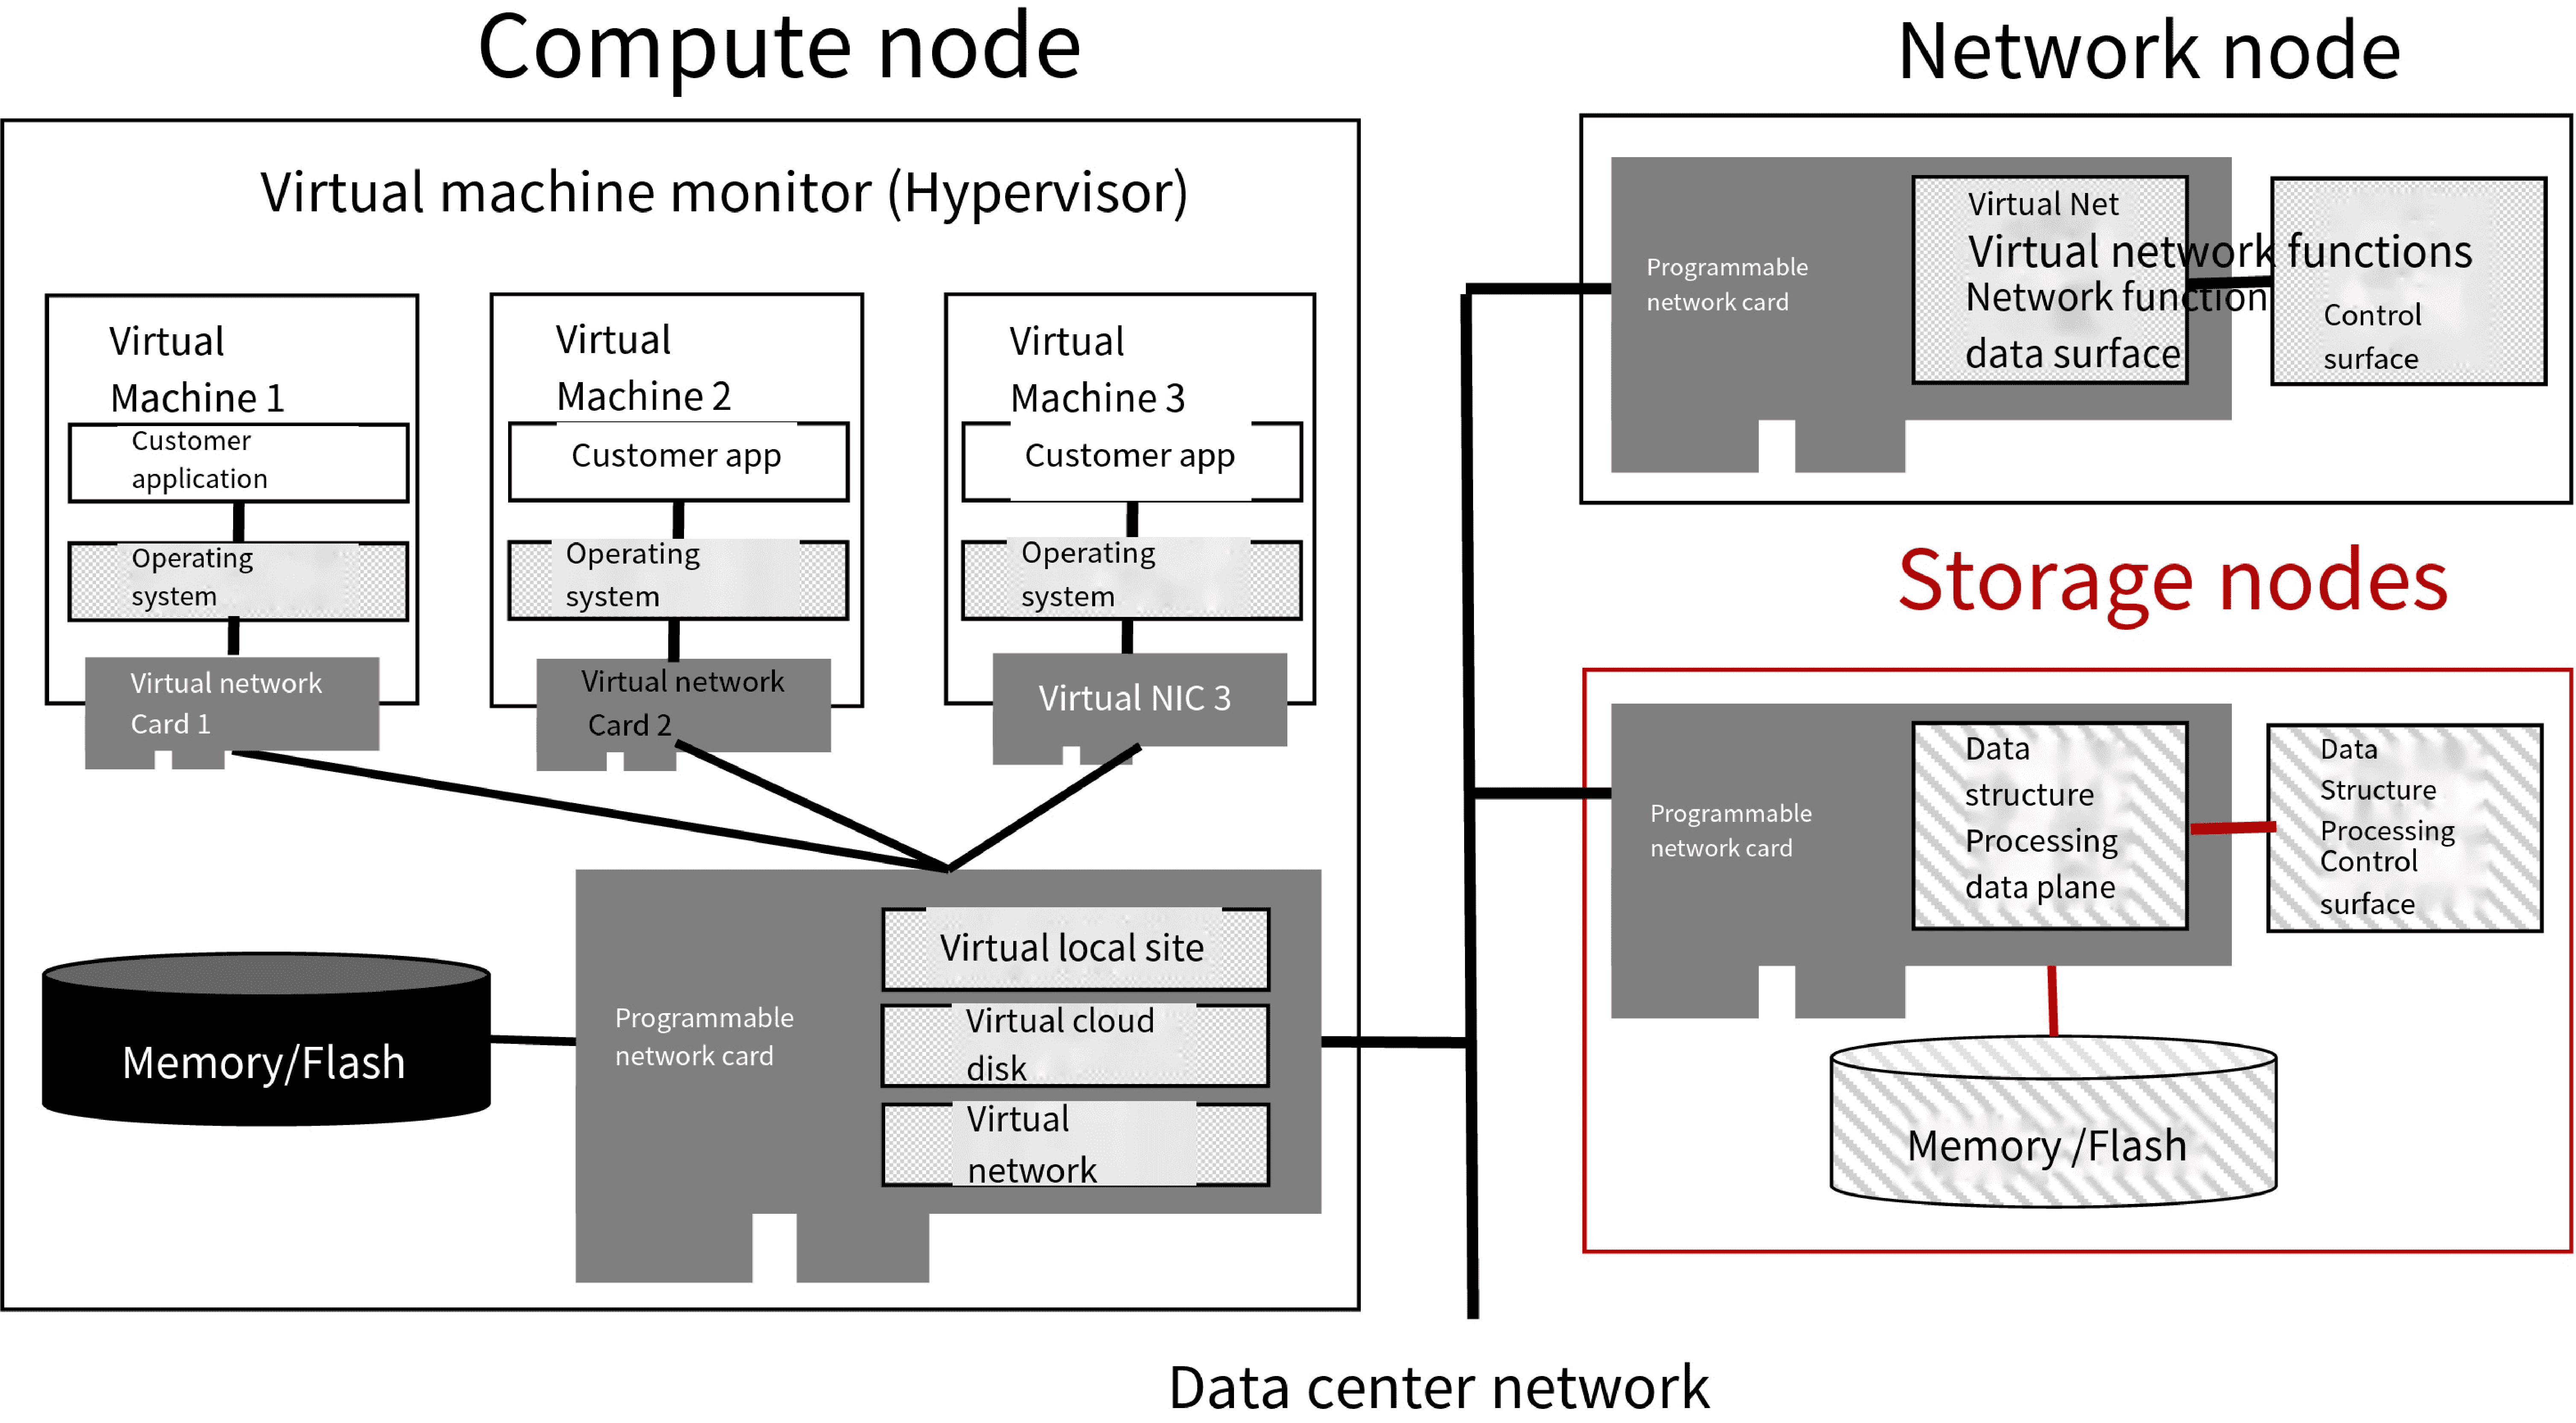
\includegraphics[width=0.8\textwidth]{figures/data_structure_accel.pdf}
	\caption{Architecture after accelerating data structure processing with a programmable network card.}
	\label{arch:fig:data-structure-accel}
\end{figure}

\section{Operating System Acceleration}

The final step is to divide the high-performance functions in the operating system into three parts, which are processed in the programmable network card, the user-mode runtime library of the host CPU, and the user-mode daemon of the host CPU, respectively.
As shown in Figure \ref{arch:fig:os-primitives-accel}, the operating system is replaced by a user-mode runtime library in the figure, and the function of the transport protocol is added in the programmable network card.
The user-mode runtime library intercepts the system calls of the application program by replacing the standard library (such as libc), so that part of the operating system functions can be implemented in user mode, and the other part of the functions can be offloaded to the programmable network card.
The user-mode daemon is mainly used for control plane operations, which are not shown in Figure \ref{arch:fig:os-primitives-accel} for simplicity.

\begin{figure}[htbp]
	\centering
	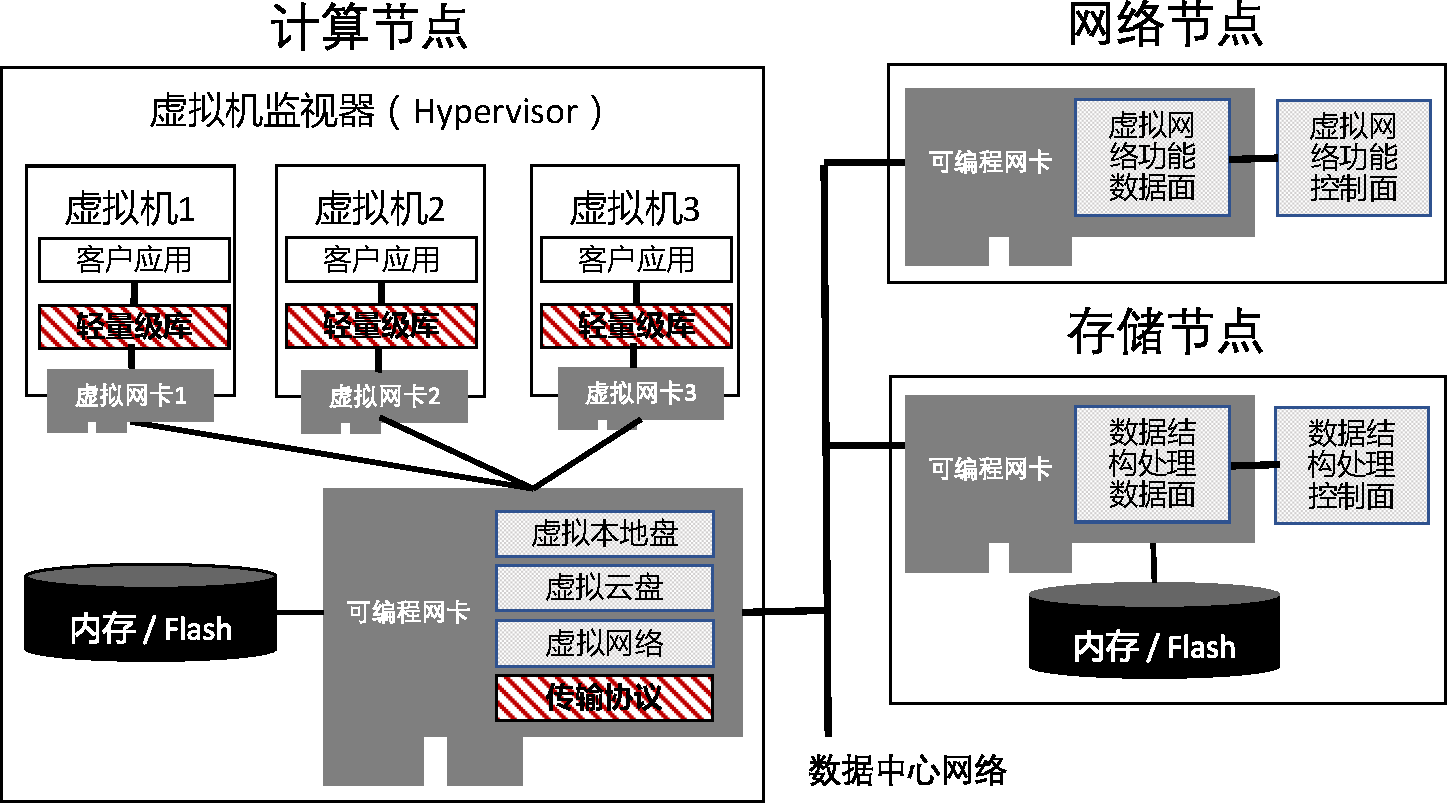
\includegraphics[width=0.8\textwidth]{figures/os_primitives_accel.pdf}
	\caption{Architecture after accelerating operating system communication primitives with a programmable network card.}
	\label{arch:fig:os-primitives-accel}
\end{figure}

The operating system includes subsystems such as communication and storage. This article takes the acceleration of the communication system as an example. The socket is the most commonly used communication primitive for application programs, but its performance is not satisfactory due to various overheads of the operating system.
Chapter \ref{chapter:socksdirect} designs and implements a high-performance user-mode socket system, which is fully compatible with existing applications, and can achieve low latency and high throughput close to the hardware limit for both intra-host process communication and cross-host communication.
The system is composed of a reliable communication protocol on the programmable network card and a user-mode library and user-mode daemon running on the host CPU.
For cross-host communication, the data plane is composed of the programmable network card and the user-mode library. The programmable network card is responsible for low-level semantics such as multiplexing and reliable transmission, and provides Remote Direct Memory Access (RDMA) primitives; the user-mode library is responsible for encapsulating RDMA primitives into the socket semantics of the Linux Virtual File System, providing high-level semantics such as lock-free message queues, buffer management, waiting events, and zero-copy memory page remapping.
For intra-host communication, the data plane is composed of the CPU's hardware memory coherence protocol and the user-mode library. The user-mode library establishes shared memory queues between processes and relies on the CPU's memory coherence protocol for automatic synchronization. The functions of the user-mode library are similar to those of cross-host communication.
The user-mode daemon is responsible for the control plane, that is, initialization, process creation and exit, connection establishment and closure, establishing queues with the RDMA network card, and establishing shared memory queues between processes.

In the design of Chapter \ref{chapter:socksdirect}, the client application accesses the RDMA function in the programmable network card directly through the SocksDirect runtime library, without going through the operating system kernel and the virtual machine monitor, so the programmable network card does not need to support SR-IOV hardware virtualization.



\section{Programmable Network Card}

After introducing the data center system architecture based on the programmable network card, this section introduces the software and hardware architecture inside the programmable network card. As shown in Figure \ref{arch:fig:sw-hw-codesign}, the logic inside the programmable network card is mainly composed of the programming framework in Chapter \ref{chapter:clicknp}, the basic service middleware in Chapter \ref{chapter:kvdirect}, and the application layer in Chapters \ref{chapter:kvdirect} and \ref{chapter:socksdirect}. The corresponding software on the host CPU includes the FPGA communication library and driver in Chapter \ref{chapter:clicknp}, the key-value operation library in Chapter \ref{chapter:kvdirect}, and the socket communication library compatible with the Linux operating system in Chapter \ref{chapter:socksdirect}.

\begin{figure}[htbp]
	\centering
	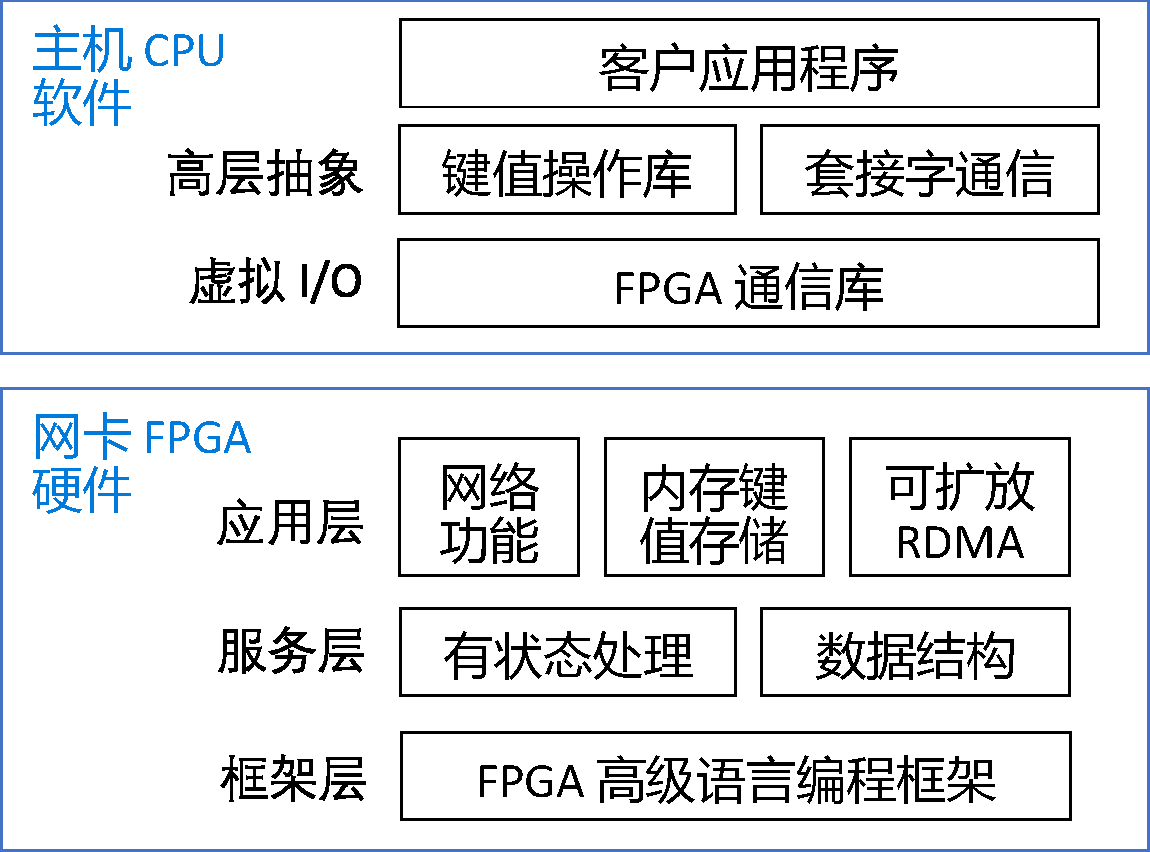
\includegraphics[width=0.5\textwidth]{figures/sw_hw_codesign.pdf}
	\caption{Programmable network card architecture with software-hardware co-design.}
	\label{arch:fig:sw-hw-codesign}
\end{figure}


Figure \ref{arch:fig:my-smartnic-current} shows the hardware architecture of the Catapult programmable network card \cite{putnam2014reconfigurable} used in this paper.
The Catapult programmable network card consists of a Stratix V FPGA and a Mellanox ConnectX-3 commercial network card. The FPGA has two QSFP interfaces connecting to the 40 Gbps Ethernet network, one connecting to the data center switch, and the other connecting to the commercial network card inside the programmable network card. Since the FPGA used in this paper does not have a PCIe Gen3 x16 hard core, the FPGA is connected to the host through two PCIe Gen3 x8 interfaces, which share a PCIe Gen3 x16 physical slot. The commercial network card has two 40 Gbps Ethernet interfaces, one connecting to the FPGA and the other idle. The commercial network card is connected to the host through a PCIe Gen3 x16 interface.

\begin{figure}[htbp]
	\centering
	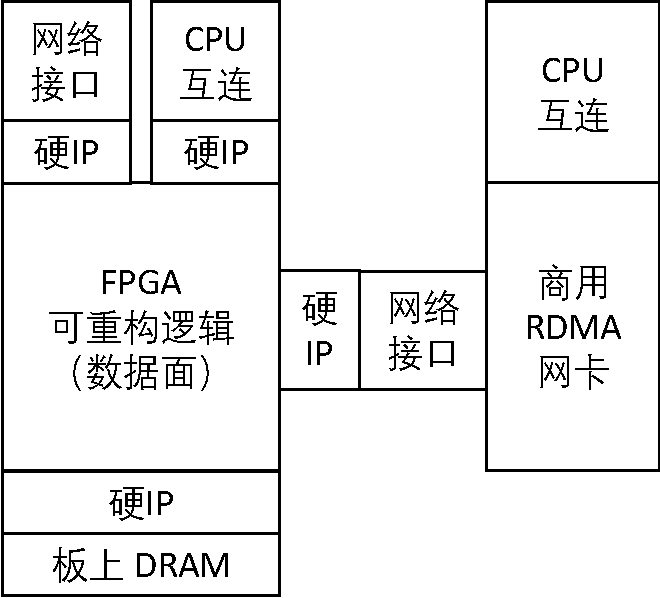
\includegraphics[width=0.4\textwidth]{figures/smartnic-current.pdf}
	\caption{The Catapult programmable network card used in this paper.}
	\label{arch:fig:my-smartnic-current}
\end{figure}

The FPGA used in this paper has 172,600 logic elements (ALM), 2,014 on-chip memories (BRAM) of 20 Kb size, and 1,590 digital signal processing units (DSP) that can perform 16-bit multiplication. The FPGA board also has 4 GB of DRAM, which is connected to the FPGA via a DDR3 channel.

Chapters \ref{chapter:clicknp} and \ref{chapter:kvdirect} of this paper use the reconfigurable logic of the FPGA to implement network functions and data structure processing; Chapter \ref{chapter:socksdirect} uses the commercial RDMA network card to implement the hardware transport protocol part of socket primitives.
Data packets from the data center network are received by the programmable network card from the network interface in the upper left corner of the FPGA. If it is a network function or data structure processing requirement, it is directly processed in the FPGA reconfigurable logic, and the FPGA needs to use the on-board DRAM and access the host DRAM through the CPU interconnect (such as PCIe) during the processing.
If the data packet is for socket communication in Chapter \ref{chapter:socksdirect}, it will be decapsulated in the FPGA's virtual network and sent to the commercial RDMA network card through the network interface between the FPGA and the commercial RDMA network card.
The commercial RDMA network card will DMA the content of the data packet to the user-space socket library on the host through the CPU interconnect (such as PCIe).

\iffalse
\textbf{Details moved to later chapters}


\subsection{High-level language programming framework}

To simplify FPGA programming, Chapter \ref{chapter:clicknp} of this paper will propose a modular FPGA high-level language programming framework ClickNP suitable for stream processing.
As shown in Figure \ref{arch:fig:element_arch}, the basic processing module of ClickNP is the element. Elements are connected by channels.
Each element is programmed in C-like language and can be compiled into a logic module on the FPGA or a thread on the CPU.
Each element can be logically compared to a CPU core, is a state machine, and consists of private internal states, global states, several input channels, several output channels, data processing functions, and signal processing functions.
The global state is implemented using on-board DRAM, and the private internal state is implemented using on-chip BRAM or registers.
The channels between logic modules on the FPGA are implemented with first-in-first-out queues (FIFO), the channels between threads on the CPU are implemented with shared memory queues, and the channels between FPGA and CPU elements are implemented with PCIe I/O channels.
The data processing function reads data from the input channel and sends it to the output channel after processing. The signal processing function is used to respond to signals from the host control program.

\begin{figure}[htbp]
	\centering
	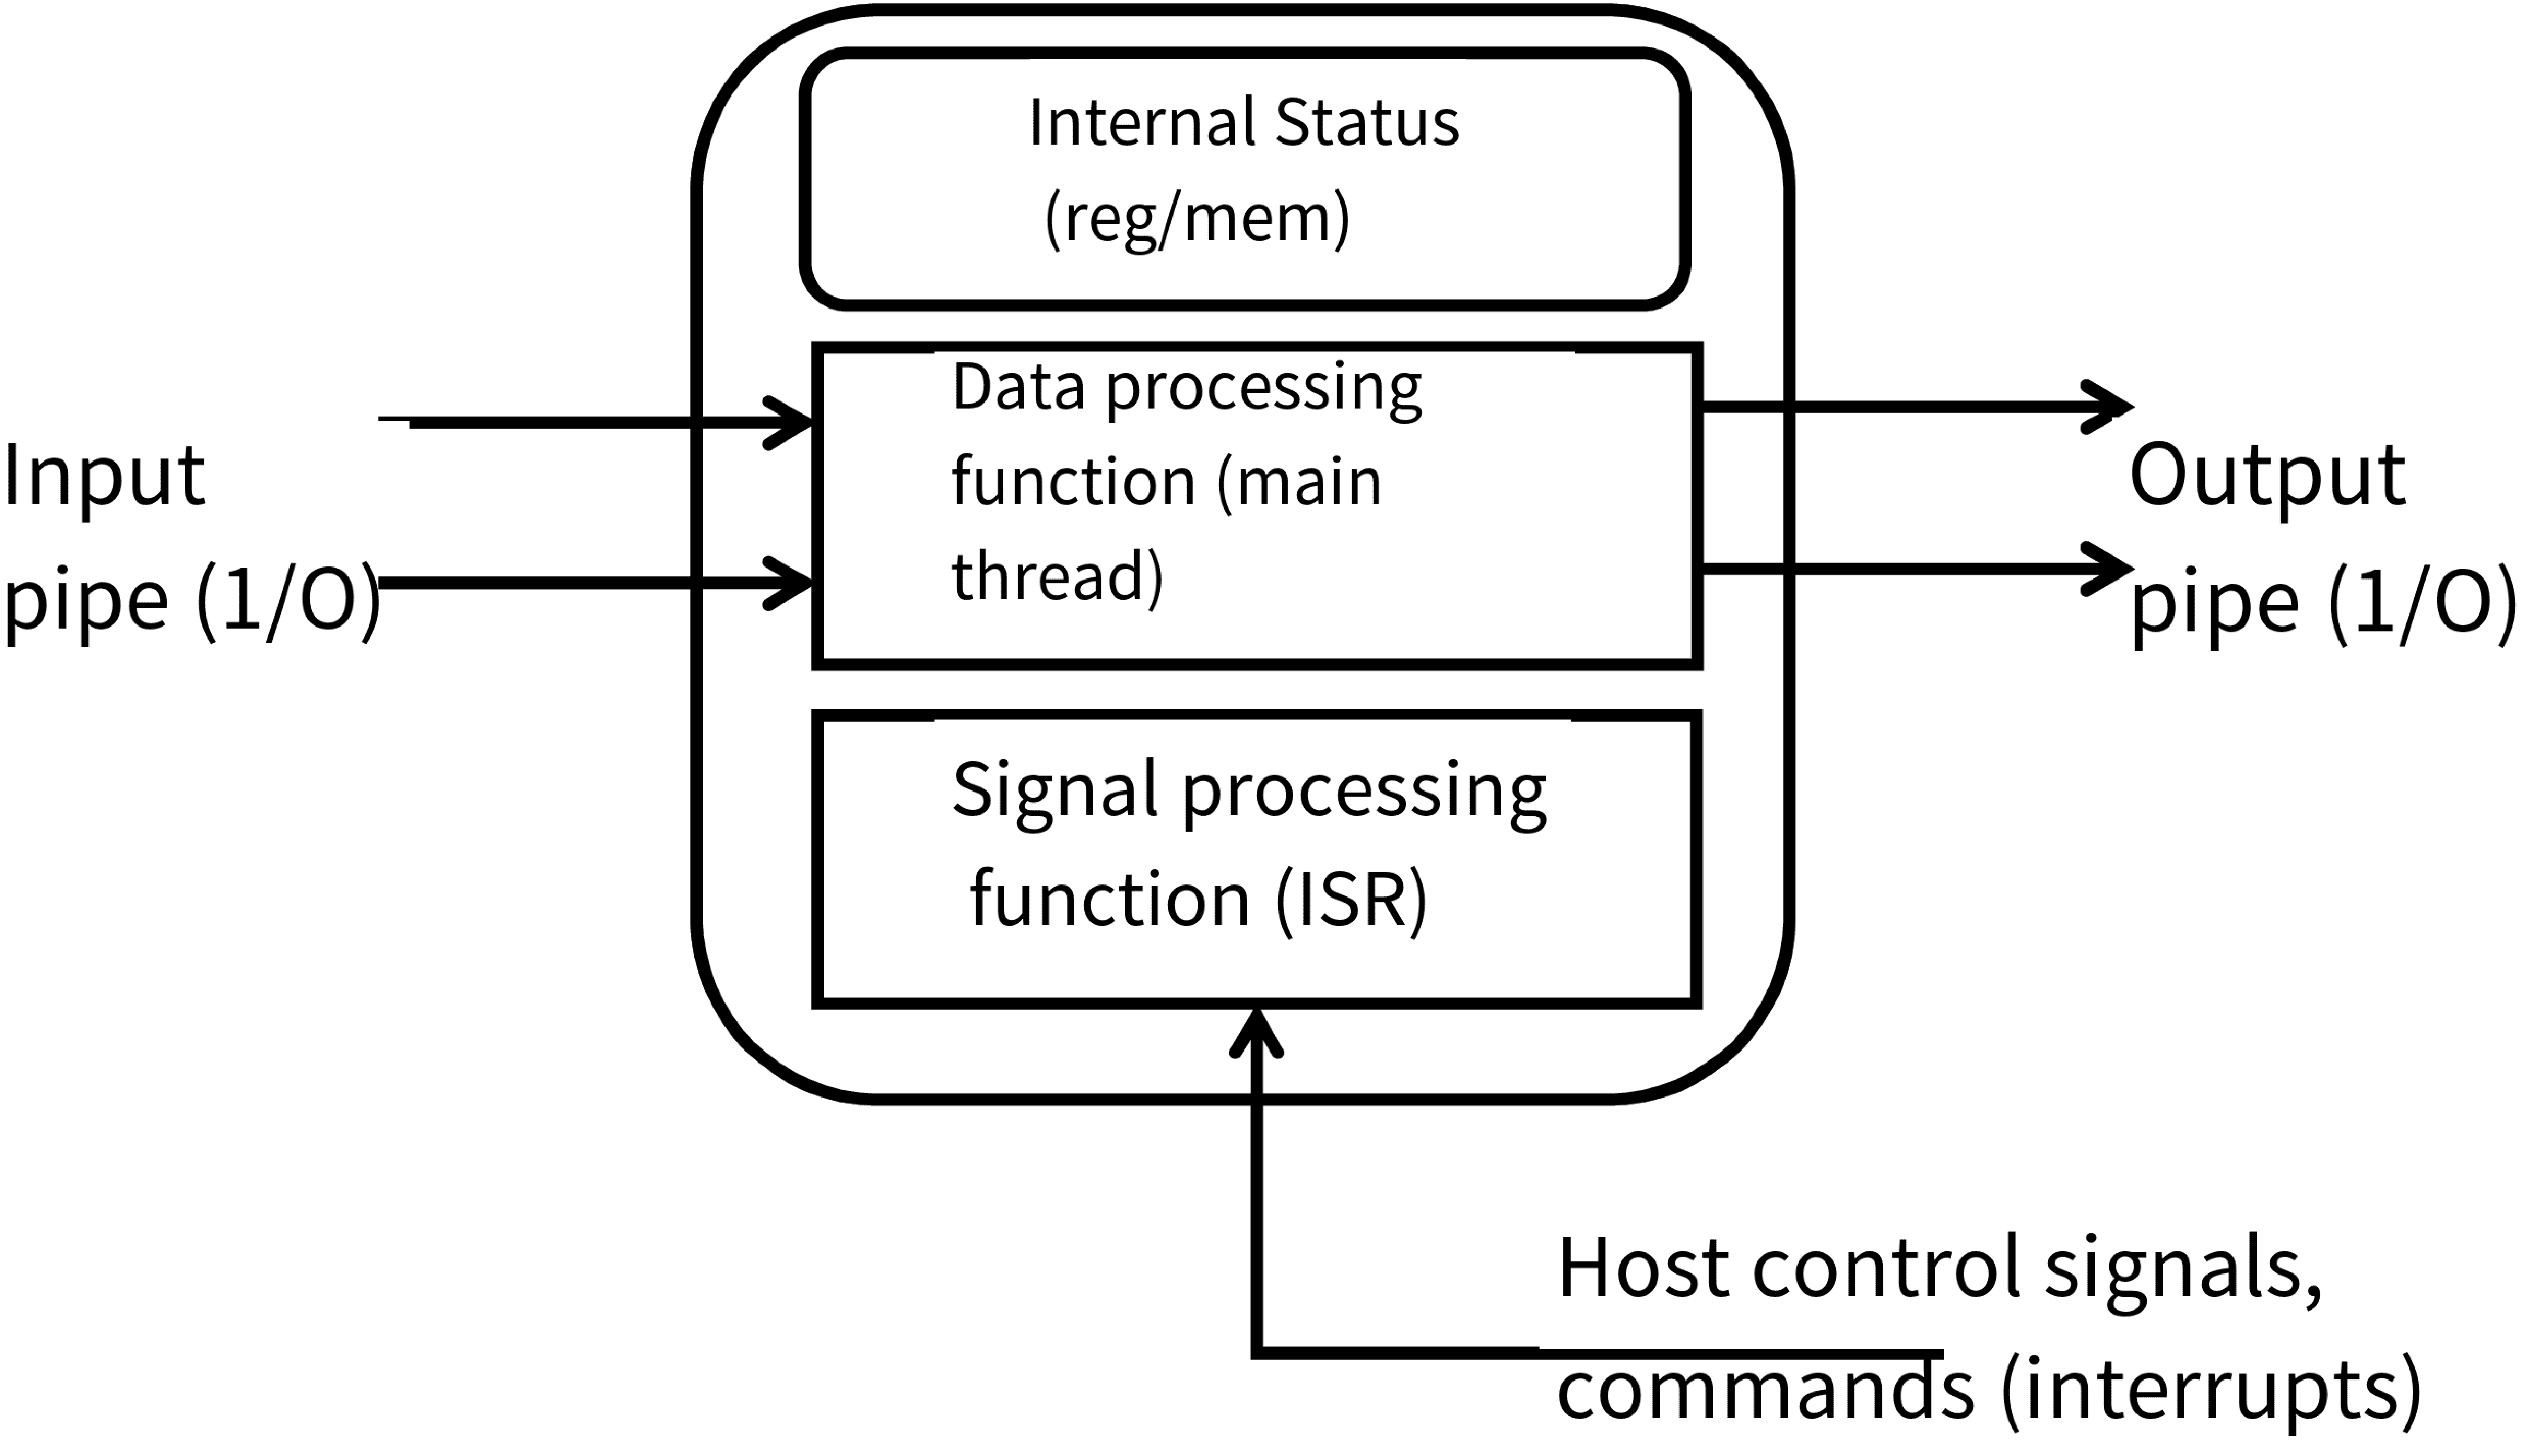
\includegraphics[width=0.5\textwidth]{chapters/clicknp/image/element_arch.pdf}
	\caption{Elements in the ClickNP programming framework.}
	\label{arch:fig:element_arch}
\end{figure}

The structure of the element enables it to implement non-blocking, fully pipelined data processing.
Not only can elements be debugged and tested on the host with traditional software development tools, but the ClickNP programming framework can also generate debugging logic for them, enabling logging, breakpoints, state queries, and other debugging functions during FPGA operation.
In addition, in live migration and high availability (HA) of virtual machines, state backup and migration in peripherals such as network cards is a challenge.
The ClickNP programming framework can automatically generate state import and export logic, and cooperate with pipeline input and output control, can achieve hot migration of elements and virtual machines through state migration, and achieve different levels of high availability of programmable network cards through hot backup or cold backup.

\subsection{Basic service middleware}

The ClickNP architecture proposed in Chapter \ref{chapter:clicknp} of this paper is more suitable for stateless or simple pipeline packet processing, but it is inadequate for processing based on connection state or application layer requests.
For example, the scheduler and hash table in the application of the four-layer load balancer are tightly coupled with the application logic, which is not easy to scale to a large number of concurrent connections, and the code maintainability is not strong. In fact, a lot of time was spent in the development process to solve the deadlock problem.
For this reason, the KV-Direct system proposed in Chapter \ref{chapter:kvdirect} of this paper will propose stateful processing and hash table data structure design within the FPGA. These basic components can serve as the basis for stateful network functions (such as four-layer load balancers) in Chapter \ref{chapter:clicknp}, memory key-value storage in Chapter \ref{chapter:kvdirect}, and scalable RDMA in Chapter \ref{chapter:socksdirect}.


For modularity and scalability, the architecture of applications on programmable network cards using KV-Direct as a basis is shown in Figure \ref{arch:fig:kvdirect_arch}.
Transactions represent dependencies, such as a connection in stateful network processing, an application layer HTTP request split across multiple packets, or operations on the same key in key-value storage.
Different requests within the same transaction need to be processed in sequence, while requests in different transactions can be processed concurrently.
To hide latency and maximize concurrent processing capabilities, the request scheduler looks up the transaction number corresponding to the request from the transaction state key-value store based on KV-Direct and queues the requests of the transactions being processed.
The data processing pipeline based on ClickNP processes according to the request data and transaction status, and may query other data structures (such as memory allocation tables, host virtual address mapping tables, firewall rule tables, routing tables, etc.) during the process.
If the request processing is completed, the response data enters the output rearrangement module, rearranges the order of the responses to meet the consistency requirements of transaction processing (for example, requests from different transactions also need to respond in the order of arrival), and finally outputs to the network.
If the processing of the request still depends on the next packet or data from the host memory DMA, in order not to block the data processing pipeline, the request will return to the scheduler, waiting for the dependent operation to complete before proceeding to the next stage of processing.

\begin{figure}[htbp]
	\centering
	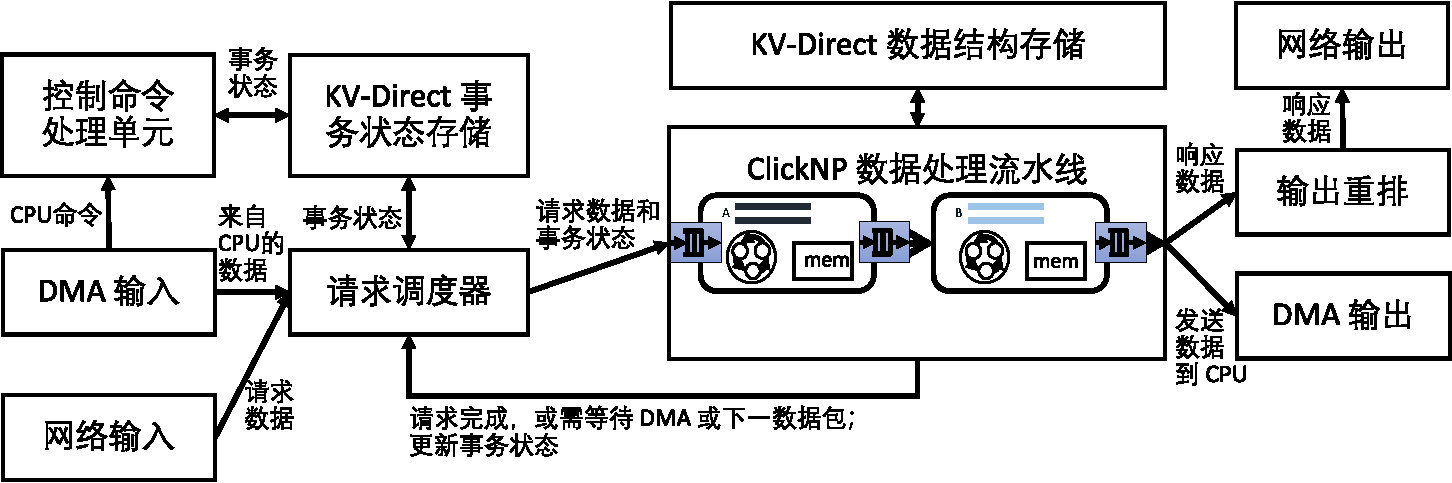
\includegraphics[width=1.0\textwidth]{figures/kvdirect_arch.pdf}
	\caption{Application layer architecture based on KV-Direct.}
	\label{arch:fig:kvdirect_arch}
\end{figure}
\fi

The next three chapters will discuss in detail the three main innovations of this paper, namely the acceleration of network functions based on programmable network cards (ClickNP), storage data structures (KV-Direct), and operating system communication primitives (SocksDirect).
